\documentclass[a4paper,12pt]{article} 

%%% Работа с русским языком
\usepackage{cmap}					% поиск в PDF
\usepackage{mathtext} 				% русские буквы в фомулах
\usepackage[T2A]{fontenc}			% кодировка
\usepackage[utf8]{inputenc}			% кодировка исходного текста
\usepackage[english,russian]{babel}	% локализация и переносы

%%% Дополнительная работа с математикой
\usepackage{amsmath,amsfonts,amssymb,amsthm,mathtools, gensymb} % AMS
\usepackage{icomma} % "Умная" запятая: $0,2$ --- число, $0, 2$ --- перечисление

%% Таблица
\usepackage[table,xcdraw]{xcolor}
\usepackage{caption}
\usepackage{subcaption}
\usepackage{floatrow}
\floatsetup[table]{capposition=top}
\floatsetup[wrapfigure]{capposition=bottom}

% Полезная штука
\usepackage{listings}

%% Номера формул
\mathtoolsset{showonlyrefs=true} % Показывать номера только у тех формул, на которые есть \eqref{} в тексте.

%% Шрифты
\usepackage{euscript}	 % Шрифт Евклид
\usepackage{mathrsfs} % Красивый матшрифт

%% Свои команды
\DeclareMathOperator{\sgn}{\mathop{sgn}}

%% Перенос знаков в формулах (по Львовскому)
\newcommand*{\hm}[1]{#1\nobreak\discretionary{}
{\hbox{$\mathsurround=0pt #1$}}{}}

%% Стиль страницы
\usepackage{fancyhdr}

%% Для рисунков
\usepackage{graphicx}
\usepackage[export]{adjustbox}
\usepackage{float}
\usepackage{ragged2e}
\usepackage{wrapfig}

%Отступы и поля 
\textwidth=20cm
\oddsidemargin=-2cm
\topmargin=-2cm
\textheight=25cm

% Цвет
\usepackage{color} %% это для отображения цвета в коде
\usepackage{listings} %% собственно, это и есть пакет listings



\pagestyle{fancy}
\begin{document}
\begin{titlepage}
\begin{center}
%\vspace*{1cm}
\large{\small ФЕДЕРАЛЬНОЕ ГОСУДАРСТВЕННОЕ АВТОНОМНОЕ ОБРАЗОВАТЕЛЬНОЕ\\ УЧРЕЖДЕНИЕ ВЫСШЕГО ОБРАЗОВАНИЯ \\ МОСКОВСКИЙ ФИЗИКО-ТЕХНИЧЕСКИЙ ИНСТИТУТ\\ (НАЦИОНАЛЬНЫЙ ИССЛЕДОВАТЕЛЬСКИЙ УНИВЕРСИТЕТ)\\ ФАКУЛЬТЕТ АЭРОКОСМИЧЕСКИХ ТЕХНОЛОГИЙ}
\vfill
\line(1,0){430}\\[1mm]
\huge{Лабораторная 6}\\
\huge\textbf{Числа с плавающей точкой (Asm)}\\
\line(1,0){430}\\[1mm]
\vfill
\begin{flushright}
\normalsize{Рогозин Владимир}\\
\normalsize{\textbf{Группа Б03-106}}\\
\end{flushright}
\end{center}
\end{titlepage}
\fancyhead[L] {Лабораторная 6}


\textbf{Пункт 1: Инициализация нецелых чисел и операции с ними}

Посмотрим как инициализируются типа $float$ и $double$. В программе ниже создаются две локальные переменные -- один $float$ и один $double$. Видим, что при инициализации значения записываются в стек через специальный регистр \%xmm0 и привычную команду $mov$, но со специальным суффиксом. Как видно из второй картинки, в ассемблерном листинге числа с плавающей точкой, так как являются всё тем же набором единиц и нулей, представляются в виде целых чисел, записанных в десятичной системе, двоичная запись которых соответствует виду, в котором хранится нецелое число в памяти (знак + порядок + мантисса). Отсюда становится ясно, почему для $float$'ов и $double$'ов нужны специальные команды -- чтобы машина понимала как именно производить операции с битами. Так как размер чисел двойной точности 64 бита, $double$ представляется двумя целыми числами (по 32 бита каждое).
\begin{figure}[H]\label{fig: Initialization float and double}
    \subfloat[Инициализация $float$ и $double$]{
    \begin{minipage}[t]{0.48\textwidth}
        \centering
        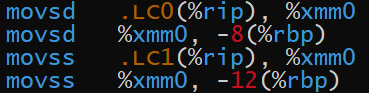
\includegraphics[width = 1\textwidth]{Присваивание float и double листинг.png}
    \end{minipage}}
    \subfloat[В представлении ассемблера]{
    \begin{minipage}[t]{0.4\textwidth}
        \centering
        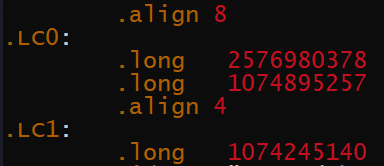
\includegraphics[width = 0.7\textwidth]{В памяти float и double листинг.png}
    \end{minipage}}
\end{figure}

Теперь арифметические операции с $float$'ами и $double$'ами. Ниже представлены две программы и их ассемблерные листинги. Можем видеть, что команды те же что и для целых чисел, но с другими суффиксами. К тому же сами числа хранятся в специальных 128-битных регистрах \%xmm0, \%xmm1 и т.д. Всего таких регистров 8 штук.
\begin{figure}[H]\label{fig: Code operations float and double}
    \subfloat[Арифм. операции $float$]{
    \begin{minipage}[t]{0.4\textwidth}
        \centering
        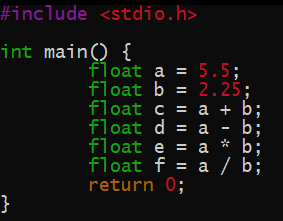
\includegraphics[width = 0.77\textwidth]{Операции float код.png}
    \end{minipage}}
    \subfloat[Арифм. операции $double$]{
    \begin{minipage}[t]{0.4\textwidth}
        \centering
        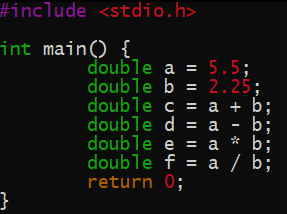
\includegraphics[width = 0.8\textwidth]{Операции double код.png}
    \end{minipage}}
\end{figure}

\begin{figure}[H]\label{fig: Listing operations float and double}
    \subfloat[Листинг $float$]{
    \begin{minipage}[t]{0.4\textwidth}
        \centering
        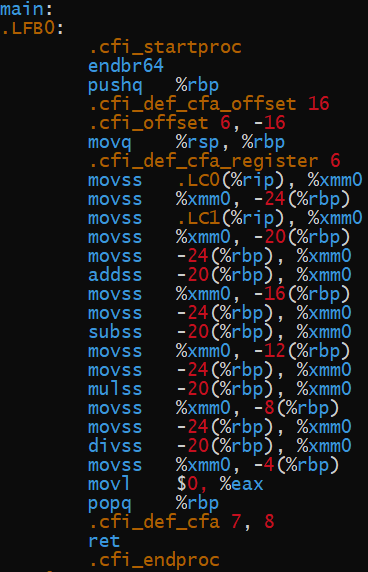
\includegraphics[width = 0.85\textwidth]{Операции float листинг.png}
    \end{minipage}}
    \subfloat[Листинг $double$]{
    \begin{minipage}[t]{0.4\textwidth}
        \centering
        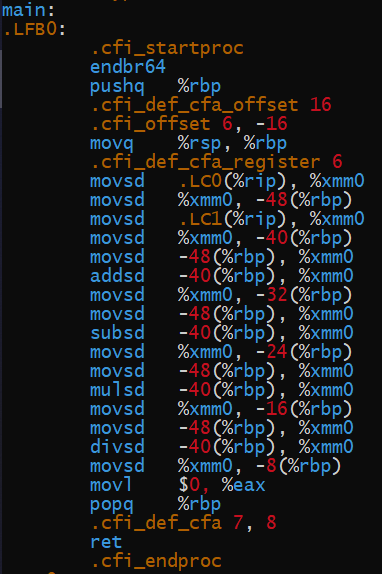
\includegraphics[width = 0.88\textwidth]{Операции double листинг.png}
    \end{minipage}}
\end{figure}

\textbf{Пункт 2: Ускоренное среднее арифметическое элементов массива}

Сначала на С++ напишем простейшую программку для вычисления среднего арифметического статического массива из $double$'ов. В цикле происходит суммирование элементов массива, после этого получившаяся сумма делится на количество элементов. Сразу посмотрим на оптимизацию O3, а точнее её листинг.
\begin{figure}[H]\label{fig: listing and code Average double}
    \subfloat[Суммирование Asm]{
    \begin{minipage}[t]{0.4\textwidth}
        \centering
        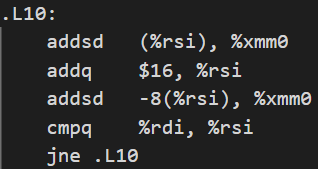
\includegraphics[width = 0.85\textwidth]{Average листинг.png}
    \end{minipage}}
    \subfloat[Суммирование C++]{
    \begin{minipage}[t]{0.4\textwidth}
        \centering
        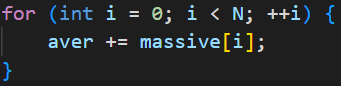
\includegraphics[width = 0.88\textwidth]{Average код.png}
    \end{minipage}}
\end{figure}
В регистре \%rsi изначально лежал адрес нулевого элемента массива. Видим, что, благодаря оптимизации, за одну итерацию происходит два сложения (компилятор сам устроил конвейер операций), но происходят они по очереди, а не одной командой. Попробуем, с помощью ассемблерной вставки, используя распараллеливание сложения при помощи SSE ещё ускорить программу. Будем складывать два числа за одну операцию, по окончании цикла получим две суммы, сложим их и получим искомую сумму. Ассемблерная вставка представлена ниже на картинке.

После этого сравним время работы программ для массивов 16,..., 16 000 000 элементов, будем находить среднее арифметическое 20 раз, каждый раз генерировать новый массив. Результаты представлены на картинках ниже.

\begin{figure}[H]\label{fig: Asm optimization code}
    \centering
    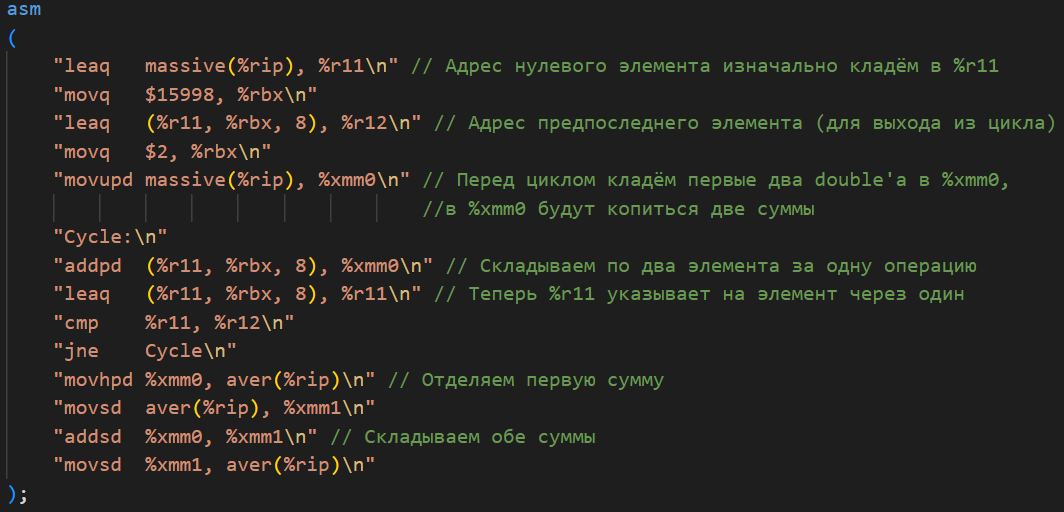
\includegraphics[width = \textwidth]{Average_optimized_Asm код.png}
    \caption{Ассемблерная вставка для ускорения работы кода}
\end{figure}

\begin{figure}[H]\label{fig: Time N = 16}
    \subfloat[$N = 16$, оптимизация O3]{
    \begin{minipage}[t]{0.4\textwidth}
        \centering
        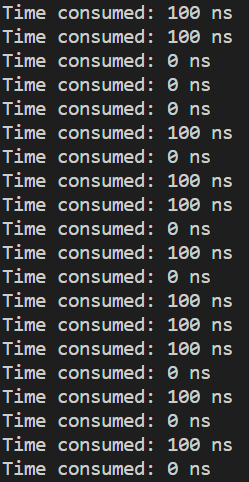
\includegraphics[width = 0.815\textwidth]{N = 16, No optimization.png}
    \end{minipage}}
    \subfloat[$N = 16$, ассемблерная вставка]{
    \begin{minipage}[t]{0.4\textwidth}
        \centering
        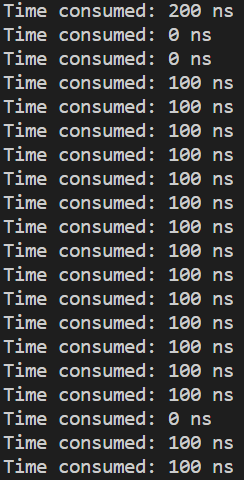
\includegraphics[width = 0.802\textwidth]{N = 16, Asm optimization.png}
    \end{minipage}}
\end{figure}

\begin{figure}[H]\label{fig: Time N = 160}
    \subfloat[$N = 160$, оптимизация O3]{
    \begin{minipage}[t]{0.4\textwidth}
        \centering
        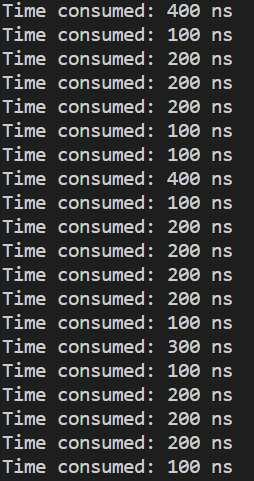
\includegraphics[width = 0.72\textwidth]{N = 160, No optimization.png}
    \end{minipage}}
    \subfloat[$N = 160$, ассемблерная вставка]{
    \begin{minipage}[t]{0.4\textwidth}
        \centering
        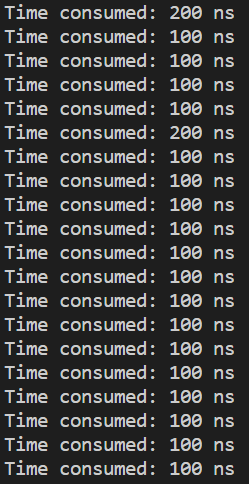
\includegraphics[width = 0.7\textwidth]{N = 160, Asm optimization.png}
    \end{minipage}}
\end{figure}

\begin{figure}[H]\label{fig: Time N = 1600}
    \subfloat[$N = 1600$, оптимизация O3]{
    \begin{minipage}[t]{0.4\textwidth}
        \centering
        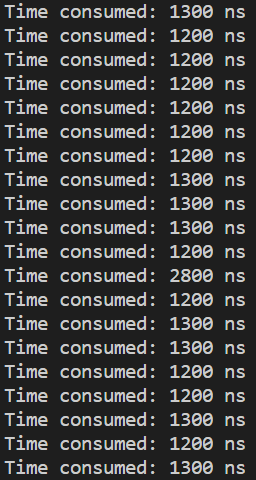
\includegraphics[width = 0.73\textwidth]{N = 1600, No optimization.png}
    \end{minipage}}
    \subfloat[$N = 1600$, ассемблерная вставка]{
    \begin{minipage}[t]{0.4\textwidth}
        \centering
        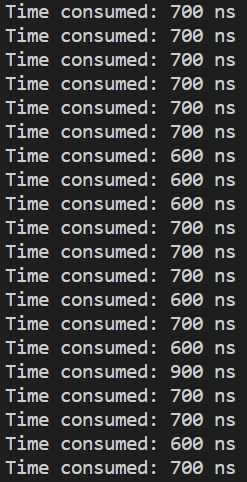
\includegraphics[width = 0.7\textwidth]{N = 1600, Asm optimization.png}
    \end{minipage}}
\end{figure}

\begin{figure}[H]\label{fig: Time N = 16000}
    \subfloat[$N = 16000$, оптимизация O3]{
    \begin{minipage}[t]{0.4\textwidth}
        \centering
        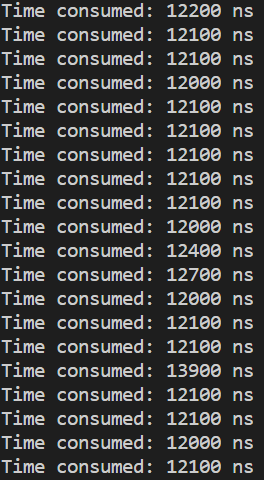
\includegraphics[width = 0.73\textwidth]{N = 16000, No optimization.png}
    \end{minipage}}
    \subfloat[$N = 16000$, ассемблерная вставка]{
    \begin{minipage}[t]{0.4\textwidth}
        \centering
        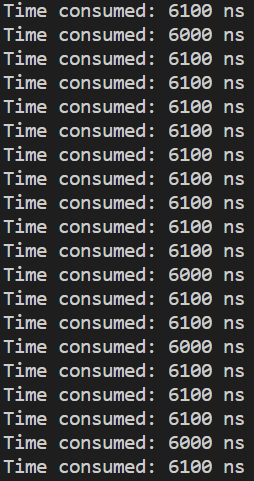
\includegraphics[width = 0.7\textwidth]{N = 16000, Asm optimization.png}
    \end{minipage}}
\end{figure}

\begin{figure}[H]\label{fig: Time N = 160000}
    \subfloat[$N = 160000$, оптимизация O3]{
    \begin{minipage}[t]{0.4\textwidth}
        \centering
        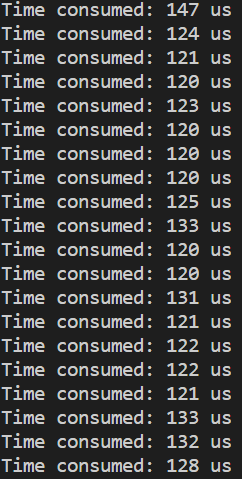
\includegraphics[width = 0.72\textwidth]{N = 160000, No optimization.png}
    \end{minipage}}
    \subfloat[$N = 160000$, ассемблерная вставка]{
    \begin{minipage}[t]{0.4\textwidth}
        \centering
        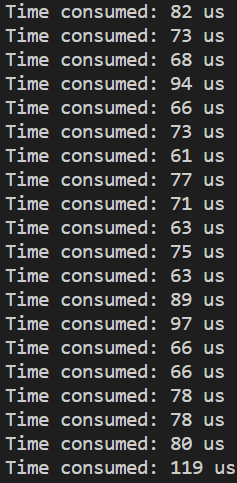
\includegraphics[width = 0.7\textwidth]{N = 160000, Asm optimization.png}
    \end{minipage}}
\end{figure}

\begin{figure}[H]\label{fig: Time N = 1600000}
    \subfloat[$N = 1600000$, оптимизация O3]{
    \begin{minipage}[t]{0.4\textwidth}
        \centering
        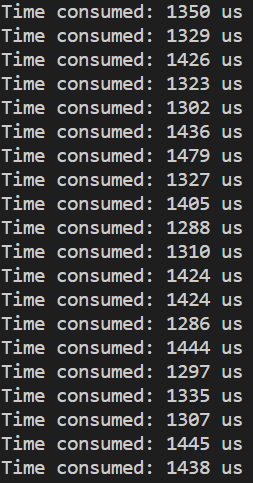
\includegraphics[width = 0.71\textwidth]{N = 1600000, No optimization.png}
    \end{minipage}}
    \subfloat[$N = 1600000$, ассемблерная вставка]{
    \begin{minipage}[t]{0.4\textwidth}
        \centering
        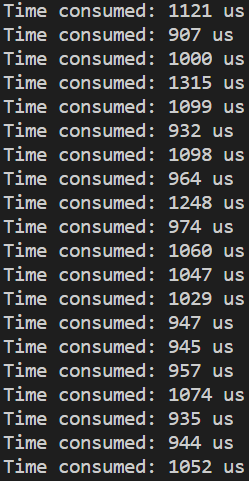
\includegraphics[width = 0.7\textwidth]{N = 1600000, Asm optimization.png}
    \end{minipage}}
\end{figure}

\begin{figure}[H]\label{fig: Time N = 16000000}
    \subfloat[$N = 16000000$, оптимизация O3]{
    \begin{minipage}[t]{0.4\textwidth}
        \centering
        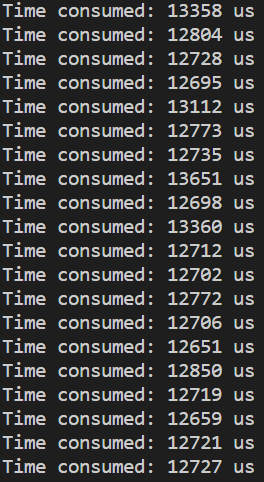
\includegraphics[width = 0.7\textwidth]{N = 16000000, No optimization.png}
    \end{minipage}}
    \subfloat[$N = 16000000$, ассемблерная вставка]{
    \begin{minipage}[t]{0.4\textwidth}
        \centering
        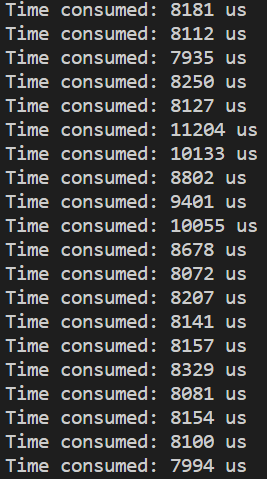
\includegraphics[width = 0.71\textwidth]{N = 16000000, Asm optimization.png}
    \end{minipage}}
\end{figure}

Занесём результаты в таблицу.
\begin{table}[H]\label{tab: No optimization vs Asm optimization Part1}
    \centering
    \begin{tabular}{|
        >{\columncolor[HTML]{FFFFFF}}c |
        >{\columncolor[HTML]{FFFFFF}}c 
        >{\columncolor[HTML]{FFFFFF}}c |
        >{\columncolor[HTML]{FFFFFF}}c 
        >{\columncolor[HTML]{FFFFFF}}c |
        >{\columncolor[HTML]{FFFFFF}}c 
        >{\columncolor[HTML]{FFFFFF}}c |
        >{\columncolor[HTML]{FFFFFF}}c 
        >{\columncolor[HTML]{FFFFFF}}c |
        >{\columncolor[HTML]{FFFFFF}}c 
        >{\columncolor[HTML]{FFFFFF}}c |}
        \hline
        {\color[HTML]{000000} } &
          \multicolumn{2}{c|}{\cellcolor[HTML]{FFFFFF}{\color[HTML]{000000} $N = 16$}} &
          \multicolumn{2}{c|}{\cellcolor[HTML]{FFFFFF}{\color[HTML]{000000} $N = 160$}} &
          \multicolumn{2}{c|}{\cellcolor[HTML]{FFFFFF}{\color[HTML]{000000} $N = 1600$}} &
          \multicolumn{2}{c|}{\cellcolor[HTML]{FFFFFF}{\color[HTML]{000000} $N = 16 \cdot 10^3$}} &
          \multicolumn{2}{c|}{\cellcolor[HTML]{FFFFFF}{\color[HTML]{000000} $N = 16 \cdot 10^4$}} \\ \hline
        {\color[HTML]{000000} №} &
          \multicolumn{1}{c|}{\cellcolor[HTML]{FFFFFF}{\color[HTML]{000000} O3, нс}} &
          {\color[HTML]{000000} SSE, нс} &
          \multicolumn{1}{c|}{\cellcolor[HTML]{FFFFFF}{\color[HTML]{000000} O3, нс}} &
          {\color[HTML]{000000} SSE, нс} &
          \multicolumn{1}{c|}{\cellcolor[HTML]{FFFFFF}{\color[HTML]{000000} O3, нс}} &
          {\color[HTML]{000000} SSE, нс} &
          \multicolumn{1}{c|}{\cellcolor[HTML]{FFFFFF}{\color[HTML]{000000} O3, нс}} &
          {\color[HTML]{000000} SSE, нс} &
          \multicolumn{1}{c|}{\cellcolor[HTML]{FFFFFF}{\color[HTML]{000000} O3, мкс}} &
          {\color[HTML]{000000} SSE, мкс} \\ \hline
        {\color[HTML]{000000} 1} &
          \multicolumn{1}{c|}{\cellcolor[HTML]{FFFFFF}{\color[HTML]{000000} 100}} &
          {\color[HTML]{000000} 200} &
          \multicolumn{1}{c|}{\cellcolor[HTML]{FFFFFF}{\color[HTML]{000000} 400}} &
          {\color[HTML]{000000} 200} &
          \multicolumn{1}{c|}{\cellcolor[HTML]{FFFFFF}{\color[HTML]{000000} 1300}} &
          {\color[HTML]{000000} 700} &
          \multicolumn{1}{c|}{\cellcolor[HTML]{FFFFFF}{\color[HTML]{000000} 12200}} &
          {\color[HTML]{000000} 6100} &
          \multicolumn{1}{c|}{\cellcolor[HTML]{FFFFFF}{\color[HTML]{000000} 147}} &
          {\color[HTML]{000000} 82} \\ \hline
        {\color[HTML]{000000} 2} &
          \multicolumn{1}{c|}{\cellcolor[HTML]{FFFFFF}{\color[HTML]{000000} 100}} &
          {\color[HTML]{000000} 0} &
          \multicolumn{1}{c|}{\cellcolor[HTML]{FFFFFF}{\color[HTML]{000000} 100}} &
          {\color[HTML]{000000} 100} &
          \multicolumn{1}{c|}{\cellcolor[HTML]{FFFFFF}{\color[HTML]{000000} 1200}} &
          {\color[HTML]{000000} 700} &
          \multicolumn{1}{c|}{\cellcolor[HTML]{FFFFFF}{\color[HTML]{000000} 12100}} &
          {\color[HTML]{000000} 6000} &
          \multicolumn{1}{c|}{\cellcolor[HTML]{FFFFFF}{\color[HTML]{000000} 124}} &
          {\color[HTML]{000000} 73} \\ \hline
        {\color[HTML]{000000} 3} &
          \multicolumn{1}{c|}{\cellcolor[HTML]{FFFFFF}{\color[HTML]{000000} 0}} &
          {\color[HTML]{000000} 0} &
          \multicolumn{1}{c|}{\cellcolor[HTML]{FFFFFF}{\color[HTML]{000000} 200}} &
          {\color[HTML]{000000} 100} &
          \multicolumn{1}{c|}{\cellcolor[HTML]{FFFFFF}{\color[HTML]{000000} 1200}} &
          {\color[HTML]{000000} 700} &
          \multicolumn{1}{c|}{\cellcolor[HTML]{FFFFFF}{\color[HTML]{000000} 12100}} &
          {\color[HTML]{000000} 6100} &
          \multicolumn{1}{c|}{\cellcolor[HTML]{FFFFFF}{\color[HTML]{000000} 121}} &
          {\color[HTML]{000000} 68} \\ \hline
        {\color[HTML]{000000} 4} &
          \multicolumn{1}{c|}{\cellcolor[HTML]{FFFFFF}{\color[HTML]{000000} 0}} &
          {\color[HTML]{000000} 100} &
          \multicolumn{1}{c|}{\cellcolor[HTML]{FFFFFF}{\color[HTML]{000000} 200}} &
          {\color[HTML]{000000} 100} &
          \multicolumn{1}{c|}{\cellcolor[HTML]{FFFFFF}{\color[HTML]{000000} 1200}} &
          {\color[HTML]{000000} 700} &
          \multicolumn{1}{c|}{\cellcolor[HTML]{FFFFFF}{\color[HTML]{000000} 12000}} &
          {\color[HTML]{000000} 6100} &
          \multicolumn{1}{c|}{\cellcolor[HTML]{FFFFFF}{\color[HTML]{000000} 120}} &
          {\color[HTML]{000000} 94} \\ \hline
        {\color[HTML]{000000} 5} &
          \multicolumn{1}{c|}{\cellcolor[HTML]{FFFFFF}{\color[HTML]{000000} 0}} &
          {\color[HTML]{000000} 100} &
          \multicolumn{1}{c|}{\cellcolor[HTML]{FFFFFF}{\color[HTML]{000000} 200}} &
          {\color[HTML]{000000} 100} &
          \multicolumn{1}{c|}{\cellcolor[HTML]{FFFFFF}{\color[HTML]{000000} 1200}} &
          {\color[HTML]{000000} 700} &
          \multicolumn{1}{c|}{\cellcolor[HTML]{FFFFFF}{\color[HTML]{000000} 12100}} &
          {\color[HTML]{000000} 6100} &
          \multicolumn{1}{c|}{\cellcolor[HTML]{FFFFFF}{\color[HTML]{000000} 123}} &
          {\color[HTML]{000000} 66} \\ \hline
        {\color[HTML]{000000} 6} &
          \multicolumn{1}{c|}{\cellcolor[HTML]{FFFFFF}{\color[HTML]{000000} 100}} &
          {\color[HTML]{000000} 100} &
          \multicolumn{1}{c|}{\cellcolor[HTML]{FFFFFF}{\color[HTML]{000000} 100}} &
          {\color[HTML]{000000} 200} &
          \multicolumn{1}{c|}{\cellcolor[HTML]{FFFFFF}{\color[HTML]{000000} 1200}} &
          {\color[HTML]{000000} 700} &
          \multicolumn{1}{c|}{\cellcolor[HTML]{FFFFFF}{\color[HTML]{000000} 12100}} &
          {\color[HTML]{000000} 6100} &
          \multicolumn{1}{c|}{\cellcolor[HTML]{FFFFFF}{\color[HTML]{000000} 120}} &
          {\color[HTML]{000000} 73} \\ \hline
        {\color[HTML]{000000} 7} &
          \multicolumn{1}{c|}{\cellcolor[HTML]{FFFFFF}{\color[HTML]{000000} 0}} &
          {\color[HTML]{000000} 100} &
          \multicolumn{1}{c|}{\cellcolor[HTML]{FFFFFF}{\color[HTML]{000000} 100}} &
          {\color[HTML]{000000} 100} &
          \multicolumn{1}{c|}{\cellcolor[HTML]{FFFFFF}{\color[HTML]{000000} 1200}} &
          {\color[HTML]{000000} 600} &
          \multicolumn{1}{c|}{\cellcolor[HTML]{FFFFFF}{\color[HTML]{000000} 12100}} &
          {\color[HTML]{000000} 6100} &
          \multicolumn{1}{c|}{\cellcolor[HTML]{FFFFFF}{\color[HTML]{000000} 120}} &
          {\color[HTML]{000000} 61} \\ \hline
        {\color[HTML]{000000} 8} &
          \multicolumn{1}{c|}{\cellcolor[HTML]{FFFFFF}{\color[HTML]{000000} 100}} &
          {\color[HTML]{000000} 100} &
          \multicolumn{1}{c|}{\cellcolor[HTML]{FFFFFF}{\color[HTML]{000000} 400}} &
          {\color[HTML]{000000} 100} &
          \multicolumn{1}{c|}{\cellcolor[HTML]{FFFFFF}{\color[HTML]{000000} 1300}} &
          {\color[HTML]{000000} 600} &
          \multicolumn{1}{c|}{\cellcolor[HTML]{FFFFFF}{\color[HTML]{000000} 12100}} &
          {\color[HTML]{000000} 6100} &
          \multicolumn{1}{c|}{\cellcolor[HTML]{FFFFFF}{\color[HTML]{000000} 120}} &
          {\color[HTML]{000000} 77} \\ \hline
        {\color[HTML]{000000} 9} &
          \multicolumn{1}{c|}{\cellcolor[HTML]{FFFFFF}{\color[HTML]{000000} 100}} &
          {\color[HTML]{000000} 100} &
          \multicolumn{1}{c|}{\cellcolor[HTML]{FFFFFF}{\color[HTML]{000000} 100}} &
          {\color[HTML]{000000} 100} &
          \multicolumn{1}{c|}{\cellcolor[HTML]{FFFFFF}{\color[HTML]{000000} 1300}} &
          {\color[HTML]{000000} 600} &
          \multicolumn{1}{c|}{\cellcolor[HTML]{FFFFFF}{\color[HTML]{000000} 12100}} &
          {\color[HTML]{000000} 6100} &
          \multicolumn{1}{c|}{\cellcolor[HTML]{FFFFFF}{\color[HTML]{000000} 125}} &
          {\color[HTML]{000000} 71} \\ \hline
    \end{tabular}
    \caption{Результаты измерений часть 1}
\end{table}
\begin{table}[H]\label{tab: No optimization vs Asm optimization Part 2.1}
    \centering
    \begin{tabular}{|
        >{\columncolor[HTML]{FFFFFF}}c |
        >{\columncolor[HTML]{FFFFFF}}c |
        >{\columncolor[HTML]{FFFFFF}}c |
        >{\columncolor[HTML]{FFFFFF}}c |
        >{\columncolor[HTML]{FFFFFF}}c |
        >{\columncolor[HTML]{FFFFFF}}c |
        >{\columncolor[HTML]{FFFFFF}}c |
        >{\columncolor[HTML]{FFFFFF}}c |
        >{\columncolor[HTML]{FFFFFF}}c |
        >{\columncolor[HTML]{FFFFFF}}c |
        >{\columncolor[HTML]{FFFFFF}}c |}
        \hline
        {\color[HTML]{000000} } &
          {\color[HTML]{000000} O3, нс} &
          {\color[HTML]{000000} SSE, нс} &
          {\color[HTML]{000000} O3, нс} &
          {\color[HTML]{000000} SSE, нс} &
          {\color[HTML]{000000} O3, нс} &
          {\color[HTML]{000000} SSE, нс} &
          {\color[HTML]{000000} O3, нс} &
          {\color[HTML]{000000} SSE, нс} &
          {\color[HTML]{000000} O3, мкс} &
          {\color[HTML]{000000} SSE, мкс} \\ \hline
        {\color[HTML]{000000} 10} &
          {\color[HTML]{000000} 0} &
          {\color[HTML]{000000} 100} &
          {\color[HTML]{000000} 200} &
          {\color[HTML]{000000} 100} &
          {\color[HTML]{000000} 1300} &
          {\color[HTML]{000000} 700} &
          {\color[HTML]{000000} 12000} &
          {\color[HTML]{000000} 6100} &
          {\color[HTML]{000000} 133} &
          {\color[HTML]{000000} 63} \\ \hline
        {\color[HTML]{000000} 11} &
          {\color[HTML]{000000} 100} &
          {\color[HTML]{000000} 100} &
          {\color[HTML]{000000} 200} &
          {\color[HTML]{000000} 100} &
          {\color[HTML]{000000} 1200} &
          {\color[HTML]{000000} 700} &
          {\color[HTML]{000000} 12400} &
          {\color[HTML]{000000} 6100} &
          {\color[HTML]{000000} 120} &
          {\color[HTML]{000000} 75} \\ \hline
        {\color[HTML]{000000} 12} &
          {\color[HTML]{000000} 0} &
          {\color[HTML]{000000} 100} &
          {\color[HTML]{000000} 200} &
          {\color[HTML]{000000} 100} &
          {\color[HTML]{000000} 2800} &
          {\color[HTML]{000000} 700} &
          {\color[HTML]{000000} 12700} &
          {\color[HTML]{000000} 6000} &
          {\color[HTML]{000000} 120} &
          {\color[HTML]{000000} 63} \\ \hline
        {\color[HTML]{000000} 13} &
          {\color[HTML]{000000} 100} &
          {\color[HTML]{000000} 100} &
          {\color[HTML]{000000} 200} &
          {\color[HTML]{000000} 100} &
          {\color[HTML]{000000} 1200} &
          {\color[HTML]{000000} 600} &
          {\color[HTML]{000000} 12000} &
          {\color[HTML]{000000} 6100} &
          {\color[HTML]{000000} 131} &
          {\color[HTML]{000000} 89} \\ \hline
        {\color[HTML]{000000} 14} &
          {\color[HTML]{000000} 100} &
          {\color[HTML]{000000} 100} &
          {\color[HTML]{000000} 100} &
          {\color[HTML]{000000} 100} &
          {\color[HTML]{000000} 1300} &
          {\color[HTML]{000000} 700} &
          {\color[HTML]{000000} 12100} &
          {\color[HTML]{000000} 6100} &
          {\color[HTML]{000000} 121} &
          {\color[HTML]{000000} 97} \\ \hline
        {\color[HTML]{000000} 15} &
          {\color[HTML]{000000} 100} &
          {\color[HTML]{000000} 100} &
          {\color[HTML]{000000} 300} &
          {\color[HTML]{000000} 100} &
          {\color[HTML]{000000} 1300} &
          {\color[HTML]{000000} 600} &
          {\color[HTML]{000000} 12100} &
          {\color[HTML]{000000} 6000} &
          {\color[HTML]{000000} 122} &
          {\color[HTML]{000000} 66} \\ \hline
        {\color[HTML]{000000} 16} &
          {\color[HTML]{000000} 0} &
          {\color[HTML]{000000} 100} &
          {\color[HTML]{000000} 100} &
          {\color[HTML]{000000} 100} &
          {\color[HTML]{000000} 1200} &
          {\color[HTML]{000000} 900} &
          {\color[HTML]{000000} 13900} &
          {\color[HTML]{000000} 6100} &
          {\color[HTML]{000000} 122} &
          {\color[HTML]{000000} 66} \\ \hline
        {\color[HTML]{000000} 17} &
          {\color[HTML]{000000} 100} &
          {\color[HTML]{000000} 100} &
          {\color[HTML]{000000} 200} &
          {\color[HTML]{000000} 100} &
          {\color[HTML]{000000} 1200} &
          {\color[HTML]{000000} 700} &
          {\color[HTML]{000000} 12100} &
          {\color[HTML]{000000} 6100} &
          {\color[HTML]{000000} 121} &
          {\color[HTML]{000000} 78} \\ \hline
        {\color[HTML]{000000} 18} &
          {\color[HTML]{000000} 0} &
          {\color[HTML]{000000} 0} &
          {\color[HTML]{000000} 200} &
          {\color[HTML]{000000} 100} &
          {\color[HTML]{000000} 1300} &
          {\color[HTML]{000000} 700} &
          {\color[HTML]{000000} 12100} &
          {\color[HTML]{000000} 6100} &
          {\color[HTML]{000000} 133} &
          {\color[HTML]{000000} 78} \\ \hline
        {\color[HTML]{000000} 19} &
          {\color[HTML]{000000} 100} &
          {\color[HTML]{000000} 100} &
          {\color[HTML]{000000} 200} &
          {\color[HTML]{000000} 100} &
          {\color[HTML]{000000} 1200} &
          {\color[HTML]{000000} 600} &
          {\color[HTML]{000000} 12000} &
          {\color[HTML]{000000} 6000} &
          {\color[HTML]{000000} 132} &
          {\color[HTML]{000000} 80} \\ \hline
        {\color[HTML]{000000} 20} &
          {\color[HTML]{000000} 0} &
          {\color[HTML]{000000} 100} &
          {\color[HTML]{000000} 100} &
          {\color[HTML]{000000} 100} &
          {\color[HTML]{000000} 1300} &
          {\color[HTML]{000000} 700} &
          {\color[HTML]{000000} 12100} &
          {\color[HTML]{000000} 6100} &
          {\color[HTML]{000000} 128} &
          {\color[HTML]{000000} 119} \\ \hline
    \end{tabular}
\end{table}

\begin{table}[H]\label{tab: No optimization vs Asm optimization Part 2.2}
    \centering
    \begin{tabular}{|
        >{\columncolor[HTML]{FFFFFF}}c |
        >{\columncolor[HTML]{FFFFFF}}c 
        >{\columncolor[HTML]{FFFFFF}}c |
        >{\columncolor[HTML]{FFFFFF}}c 
        >{\columncolor[HTML]{FFFFFF}}c |
        >{\columncolor[HTML]{FFFFFF}}c |
        >{\columncolor[HTML]{FFFFFF}}c 
        >{\columncolor[HTML]{FFFFFF}}c |
        >{\columncolor[HTML]{FFFFFF}}c 
        >{\columncolor[HTML]{FFFFFF}}c |}
        \hline
        {\color[HTML]{000000} } &
          \multicolumn{2}{c|}{\cellcolor[HTML]{FFFFFF}{\color[HTML]{000000} $N = 16 \cdot 10^5$}} &
          \multicolumn{2}{c|}{\cellcolor[HTML]{FFFFFF}{\color[HTML]{000000} $N = 16 \cdot 10^6$}} &
          {\color[HTML]{000000} } &
          \multicolumn{2}{c|}{\cellcolor[HTML]{FFFFFF}{\color[HTML]{000000} $N = 16 \cdot 10^5$}} &
          \multicolumn{2}{c|}{\cellcolor[HTML]{FFFFFF}{\color[HTML]{000000} $N = 16 \cdot 10^6$}} \\ \hline
        {\color[HTML]{000000} №} &
          \multicolumn{1}{c|}{\cellcolor[HTML]{FFFFFF}{\color[HTML]{000000} O3, мкс}} &
          {\color[HTML]{000000} SSE, мкс} &
          \multicolumn{1}{c|}{\cellcolor[HTML]{FFFFFF}{\color[HTML]{000000} O3, мкс}} &
          {\color[HTML]{000000} SSE, мкс} &
          {\color[HTML]{000000} №} &
          \multicolumn{1}{c|}{\cellcolor[HTML]{FFFFFF}{\color[HTML]{000000} O3, мкс}} &
          {\color[HTML]{000000} SSE, мкс} &
          \multicolumn{1}{c|}{\cellcolor[HTML]{FFFFFF}{\color[HTML]{000000} O3, мкс}} &
          {\color[HTML]{000000} SSE, мкс} \\ \hline
        {\color[HTML]{000000} 1} &
          \multicolumn{1}{c|}{\cellcolor[HTML]{FFFFFF}{\color[HTML]{000000} 1350}} &
          {\color[HTML]{000000} 1121} &
          \multicolumn{1}{c|}{\cellcolor[HTML]{FFFFFF}{\color[HTML]{000000} 13358}} &
          {\color[HTML]{000000} 8181} &
          {\color[HTML]{000000} 11} &
          \multicolumn{1}{c|}{\cellcolor[HTML]{FFFFFF}{\color[HTML]{000000} 1310}} &
          {\color[HTML]{000000} 1060} &
          \multicolumn{1}{c|}{\cellcolor[HTML]{FFFFFF}{\color[HTML]{000000} 12712}} &
          {\color[HTML]{000000} 8678} \\ \hline
        {\color[HTML]{000000} 2} &
          \multicolumn{1}{c|}{\cellcolor[HTML]{FFFFFF}{\color[HTML]{000000} 1329}} &
          {\color[HTML]{000000} 907} &
          \multicolumn{1}{c|}{\cellcolor[HTML]{FFFFFF}{\color[HTML]{000000} 12804}} &
          {\color[HTML]{000000} 8112} &
          {\color[HTML]{000000} 12} &
          \multicolumn{1}{c|}{\cellcolor[HTML]{FFFFFF}{\color[HTML]{000000} 1424}} &
          {\color[HTML]{000000} 1047} &
          \multicolumn{1}{c|}{\cellcolor[HTML]{FFFFFF}{\color[HTML]{000000} 12702}} &
          {\color[HTML]{000000} 8072} \\ \hline
        {\color[HTML]{000000} 3} &
          \multicolumn{1}{c|}{\cellcolor[HTML]{FFFFFF}{\color[HTML]{000000} 1426}} &
          {\color[HTML]{000000} 1000} &
          \multicolumn{1}{c|}{\cellcolor[HTML]{FFFFFF}{\color[HTML]{000000} 12728}} &
          {\color[HTML]{000000} 7935} &
          {\color[HTML]{000000} 13} &
          \multicolumn{1}{c|}{\cellcolor[HTML]{FFFFFF}{\color[HTML]{000000} 1424}} &
          {\color[HTML]{000000} 1029} &
          \multicolumn{1}{c|}{\cellcolor[HTML]{FFFFFF}{\color[HTML]{000000} 12772}} &
          {\color[HTML]{000000} 8207} \\ \hline
        {\color[HTML]{000000} 4} &
          \multicolumn{1}{c|}{\cellcolor[HTML]{FFFFFF}{\color[HTML]{000000} 1323}} &
          {\color[HTML]{000000} 1315} &
          \multicolumn{1}{c|}{\cellcolor[HTML]{FFFFFF}{\color[HTML]{000000} 12695}} &
          {\color[HTML]{000000} 8250} &
          {\color[HTML]{000000} 14} &
          \multicolumn{1}{c|}{\cellcolor[HTML]{FFFFFF}{\color[HTML]{000000} 1286}} &
          {\color[HTML]{000000} 947} &
          \multicolumn{1}{c|}{\cellcolor[HTML]{FFFFFF}{\color[HTML]{000000} 12706}} &
          {\color[HTML]{000000} 8141} \\ \hline
        {\color[HTML]{000000} 5} &
          \multicolumn{1}{c|}{\cellcolor[HTML]{FFFFFF}{\color[HTML]{000000} 1302}} &
          {\color[HTML]{000000} 1099} &
          \multicolumn{1}{c|}{\cellcolor[HTML]{FFFFFF}{\color[HTML]{000000} 13112}} &
          {\color[HTML]{000000} 8127} &
          {\color[HTML]{000000} 15} &
          \multicolumn{1}{c|}{\cellcolor[HTML]{FFFFFF}{\color[HTML]{000000} 1444}} &
          {\color[HTML]{000000} 945} &
          \multicolumn{1}{c|}{\cellcolor[HTML]{FFFFFF}{\color[HTML]{000000} 12651}} &
          {\color[HTML]{000000} 8157} \\ \hline
        {\color[HTML]{000000} 6} &
          \multicolumn{1}{c|}{\cellcolor[HTML]{FFFFFF}{\color[HTML]{000000} 1436}} &
          {\color[HTML]{000000} 932} &
          \multicolumn{1}{c|}{\cellcolor[HTML]{FFFFFF}{\color[HTML]{000000} 12773}} &
          {\color[HTML]{000000} 11204} &
          {\color[HTML]{000000} 16} &
          \multicolumn{1}{c|}{\cellcolor[HTML]{FFFFFF}{\color[HTML]{000000} 1297}} &
          {\color[HTML]{000000} 957} &
          \multicolumn{1}{c|}{\cellcolor[HTML]{FFFFFF}{\color[HTML]{000000} 12850}} &
          {\color[HTML]{000000} 8329} \\ \hline
        {\color[HTML]{000000} 7} &
          \multicolumn{1}{c|}{\cellcolor[HTML]{FFFFFF}{\color[HTML]{000000} 1479}} &
          {\color[HTML]{000000} 1098} &
          \multicolumn{1}{c|}{\cellcolor[HTML]{FFFFFF}{\color[HTML]{000000} 12735}} &
          {\color[HTML]{000000} 10133} &
          {\color[HTML]{000000} 17} &
          \multicolumn{1}{c|}{\cellcolor[HTML]{FFFFFF}{\color[HTML]{000000} 1335}} &
          {\color[HTML]{000000} 1074} &
          \multicolumn{1}{c|}{\cellcolor[HTML]{FFFFFF}{\color[HTML]{000000} 12719}} &
          {\color[HTML]{000000} 8081} \\ \hline
        {\color[HTML]{000000} 8} &
          \multicolumn{1}{c|}{\cellcolor[HTML]{FFFFFF}{\color[HTML]{000000} 1327}} &
          {\color[HTML]{000000} 964} &
          \multicolumn{1}{c|}{\cellcolor[HTML]{FFFFFF}{\color[HTML]{000000} 13651}} &
          {\color[HTML]{000000} 8802} &
          {\color[HTML]{000000} 18} &
          \multicolumn{1}{c|}{\cellcolor[HTML]{FFFFFF}{\color[HTML]{000000} 1307}} &
          {\color[HTML]{000000} 935} &
          \multicolumn{1}{c|}{\cellcolor[HTML]{FFFFFF}{\color[HTML]{000000} 12659}} &
          {\color[HTML]{000000} 8154} \\ \hline
        {\color[HTML]{000000} 9} &
          \multicolumn{1}{c|}{\cellcolor[HTML]{FFFFFF}{\color[HTML]{000000} 1405}} &
          {\color[HTML]{000000} 1248} &
          \multicolumn{1}{c|}{\cellcolor[HTML]{FFFFFF}{\color[HTML]{000000} 12698}} &
          {\color[HTML]{000000} 9401} &
          {\color[HTML]{000000} 19} &
          \multicolumn{1}{c|}{\cellcolor[HTML]{FFFFFF}{\color[HTML]{000000} 1445}} &
          {\color[HTML]{000000} 944} &
          \multicolumn{1}{c|}{\cellcolor[HTML]{FFFFFF}{\color[HTML]{000000} 12721}} &
          {\color[HTML]{000000} 8100} \\ \hline
        {\color[HTML]{000000} 10} &
          \multicolumn{1}{c|}{\cellcolor[HTML]{FFFFFF}{\color[HTML]{000000} 1288}} &
          {\color[HTML]{000000} 974} &
          \multicolumn{1}{c|}{\cellcolor[HTML]{FFFFFF}{\color[HTML]{000000} 13360}} &
          {\color[HTML]{000000} 10055} &
          {\color[HTML]{000000} 20} &
          \multicolumn{1}{c|}{\cellcolor[HTML]{FFFFFF}{\color[HTML]{000000} 1438}} &
          {\color[HTML]{000000} 1052} &
          \multicolumn{1}{c|}{\cellcolor[HTML]{FFFFFF}{\color[HTML]{000000} 12727}} &
          {\color[HTML]{000000} 7994} \\ \hline
    \end{tabular}
    \caption{Результаты измерений часть 2}
\end{table}

При достаточно больших размерах массива ($N > 1000$) программа с ассемблерной вставкой работает заметно быстрее, при малых $N$ обе работают примерно одинаково.\newpage
\textbf{Пункт 3: Среднее время работы вычисления знака числа $\pi$}

В этом пункте посмотрим на точность вычисления числа $\pi$ от времени работы программы. Формулы 3 и 4 из предыдущей лабораторной почти сразу же дают точность порядка $\sim 10^{-16}$ (с 25-ой и 30-ой итерации соответственно), формула 5 даёт неверный результат с определённого момента, поэтому будем строить графики только для первых двух (Формула Лейбница и Формула Валлиса).    
\begin{figure}[H]\label{fig: Pi_1and2_Accuracy(time)}
    \centering
    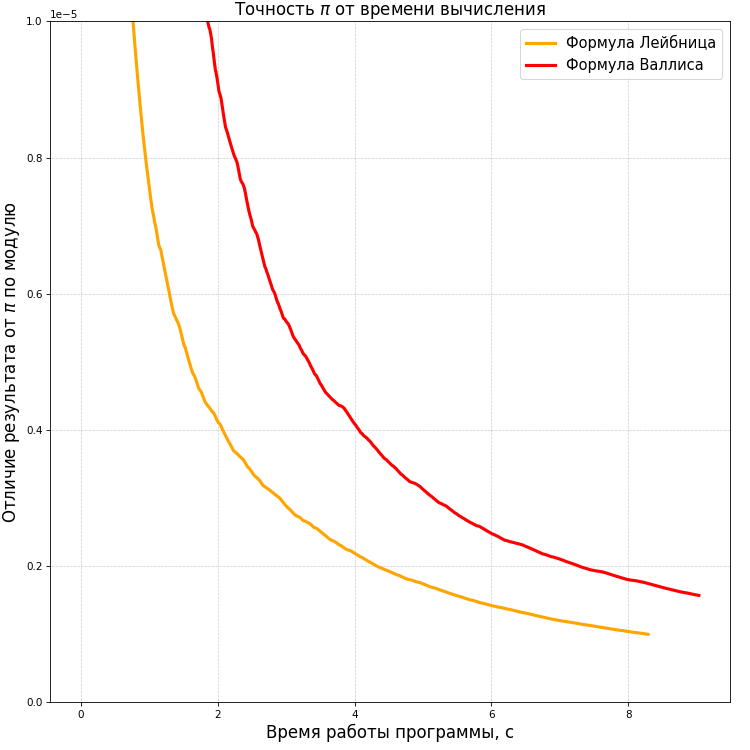
\includegraphics[width = \textwidth]{Pi_1and2_Accuracy(time).png}
\end{figure}
Из графика видно, что порядка 8-ми секунд требуется первой формуле для получения точности порядка $\sim 10^{-6}$ и 9-ти секунд требуется второй.

\textbf{Пункт 4: Ускорение вычисления среднего арифметического с помощью конвейера операций на С++}

Теперь попробуем ускорить процесс нахождения среднего арифметического, немного иначе суммируя элементы множества. Так как инструкции для основного процессора и сопроцессора могут выполняться одновременно, то есть смысл попытаться сделать так, чтобы за одну итерацию математический сопроцессор выполнял столько же действий, сколько и основной. При таком раскладе потребуется меньше итераций, и при этом время, затрачиваемое на одной итерации, не увеличится, потому что основному процессору все равно потребуется сделать столько же операций за одну итерацию. Будем применять такую оптимизацию к задаче о нахождении среднего арифметического массива элементов. 
\begin{figure}[H]\label{fig: 1sum and 2sum}
    \subfloat[Одна сумма]{
    \begin{minipage}[t]{0.4\textwidth}
        \centering
        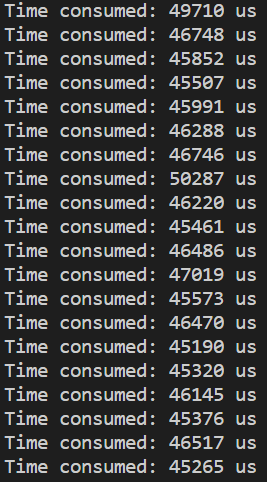
\includegraphics[width = 0.65\textwidth]{Optimized C++ 1sum.png}
    \end{minipage}}
    \subfloat[Две суммы]{
    \begin{minipage}[t]{0.4\textwidth}
        \centering
        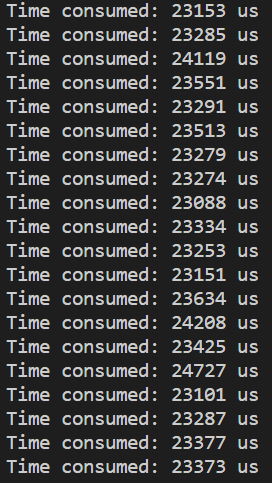
\includegraphics[width = 0.65\textwidth]{Optimized C++ 2sum.png}
    \end{minipage}}
\end{figure}
\begin{figure}[H]\label{fig: 3sum and 4sum}
    \subfloat[Три суммы]{
    \begin{minipage}[t]{0.4\textwidth}
        \centering
        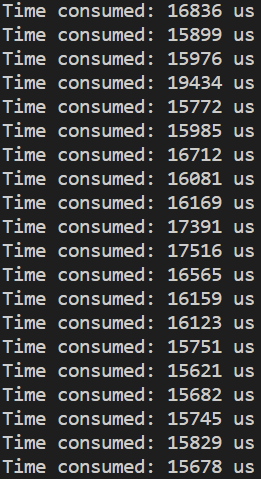
\includegraphics[width = 0.65\textwidth]{Optimized C++ 3sum.png}
    \end{minipage}}
    \subfloat[Четыре суммы]{
    \begin{minipage}[t]{0.4\textwidth}
        \centering
        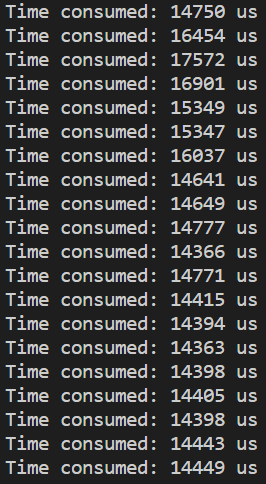
\includegraphics[width = 0.65\textwidth]{Optimized C++ 4sum.png}
    \end{minipage}}
\end{figure}

\begin{figure}[H]\label{fig: 5sum and 6sum}
    \subfloat[Пять сумм]{
    \begin{minipage}[t]{0.4\textwidth}
        \centering
        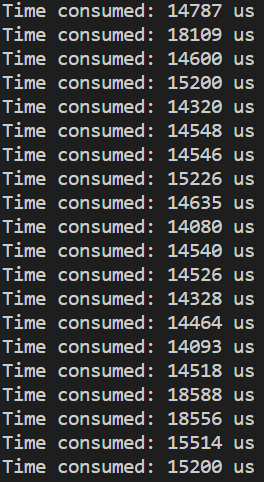
\includegraphics[width = 0.65\textwidth]{Optimized C++ 5sum.png}
    \end{minipage}}
    \subfloat[Шесть сумм]{
    \begin{minipage}[t]{0.4\textwidth}
        \centering
        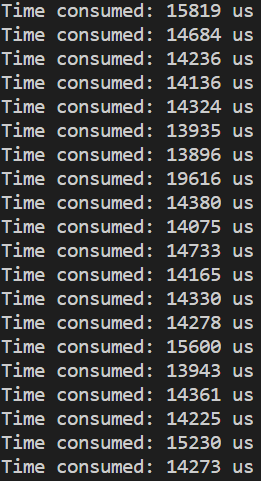
\includegraphics[width = 0.65\textwidth]{Optimized C++ 6sum.png}
    \end{minipage}}
\end{figure}
До определённого момента создавать суммы выгодно, затем время работы практически не меняется.

\textbf{Пункт 5: }

Теперь попробуем ускорить вычисление числа $\pi$ из пункта 3 с помощью конвейера операций и отключения денормализованных чисел. Сделаем две суммы и два произведения в случае первой и второй формул соответственно. Ниже представлен получившийся график.
\begin{figure}[H]\label{fig: Pi_1and2_Accuracy(time)_optimized}
    \centering
    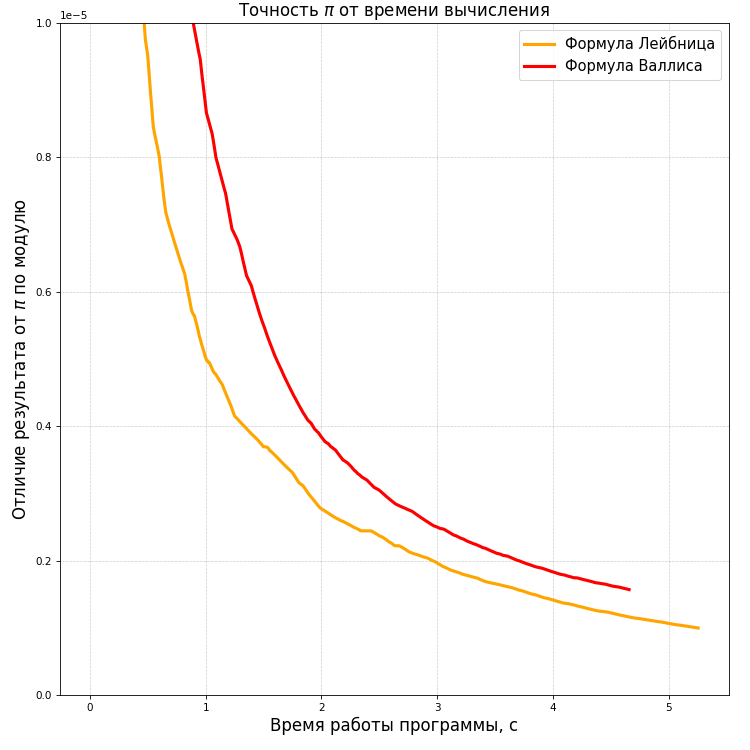
\includegraphics[width = \textwidth]{Pi_1and2_Accuracy(time)_optimized.png}
\end{figure}
Как видно, время работы заметно уменьшилось с 8-ми до примерно 5-ти секунд для заданной точности $\sim 10^{-6}$, и это только при двух суммах/произведениях, вероятно, вычисление можно ещё ускорить, подобрав оптимальное количество операций сложения/умножения за одну итерацию. Одно только отключение денормализованных чисел ускоряет вычисление на $\sim 0,3$ секунды, весь остальной эффект достигается с помощью конвейера операций. 

\end{document}

